\section{Feldeffekt-Transistoren}

\subsection{FET-Typen und Symbole}

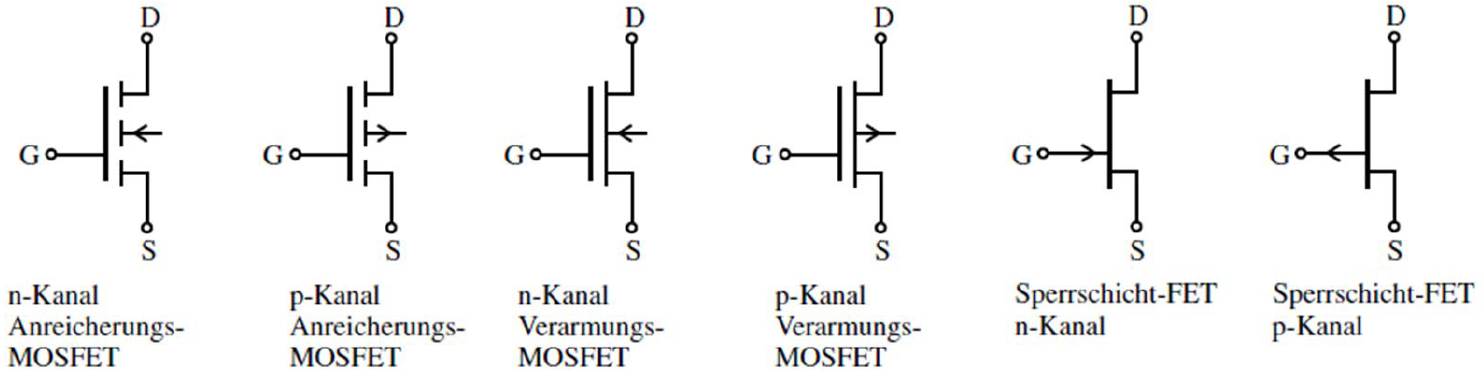
\includegraphics[align=t, width=\columnwidth]{images/fet_symbole_typen.png}


\subsubsection{Anschlüsse eines FET}

Kanal von \textbf{D}rain zu \textbf{S}ource (Stromfluss), gesteuert von \textbf{G}ate (und Bulk)


\subsection{Sperrschicht-FET / Junction FET (JFET)}

\subsubsection{Kennlinien}

\begin{minipage}[t]{0.43\columnwidth}
    \centering \textbf{Eingangskennlinie} \\
    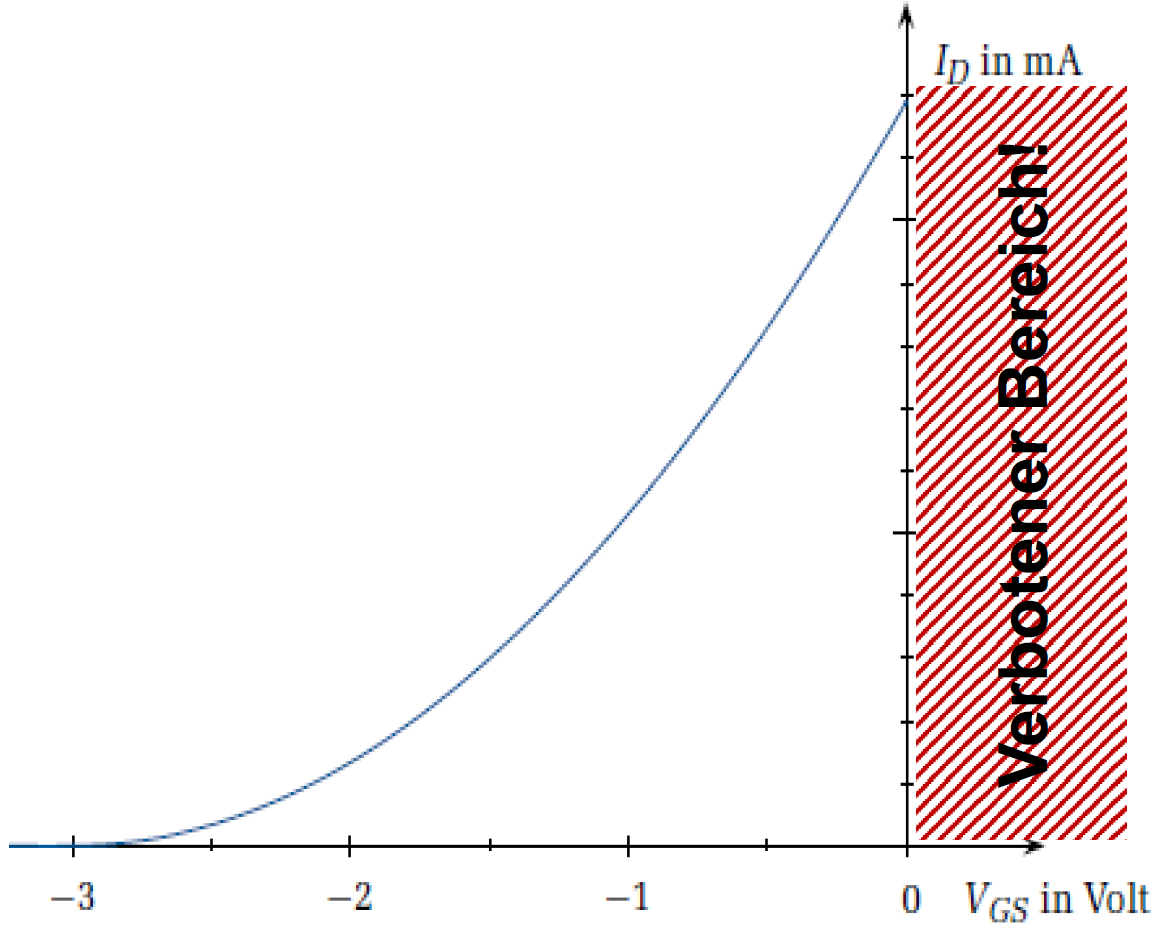
\includegraphics[align=c, width=\columnwidth]{images/jfet_eingangskennlinie.png}
\end{minipage}
\hfill
\begin{minipage}[t]{0.54\columnwidth}
    \textbf{Ausgangskennlinien} \\
    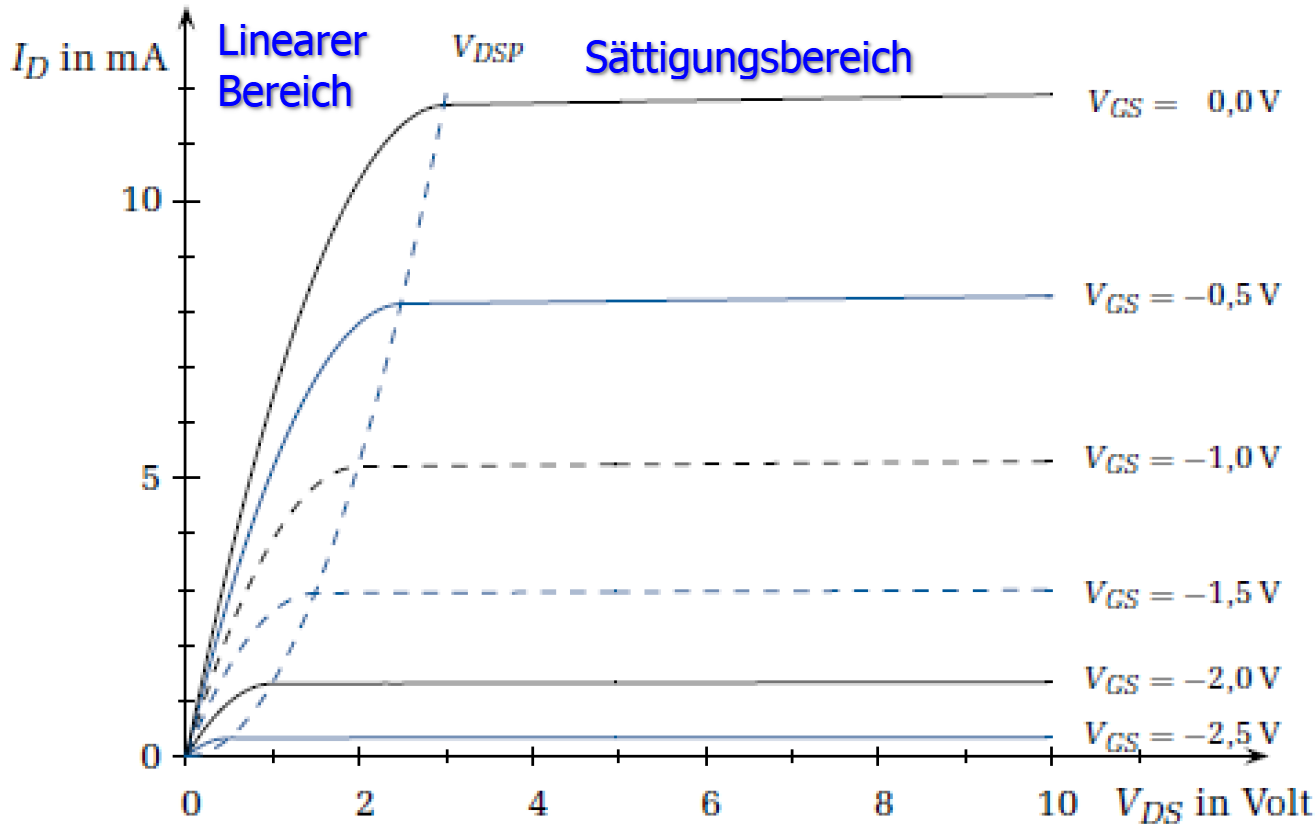
\includegraphics[align=c, width=\columnwidth]{images/jfet_ausgangskennlinien.png}
\end{minipage}


\subsubsection{Linearer Bereich (gesteuerter Widerstand)}

\begin{minipage}[t]{0.3\columnwidth}
    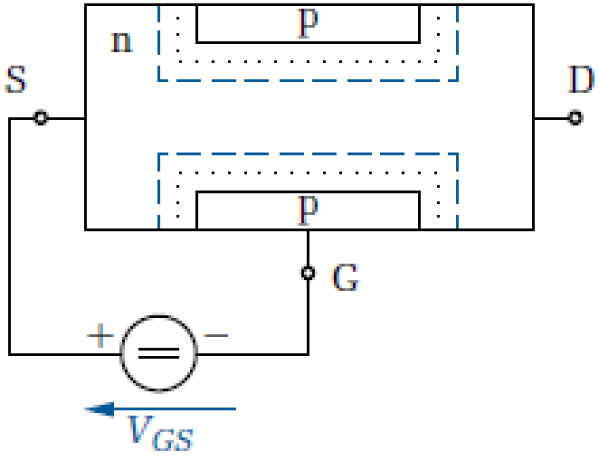
\includegraphics[align=t, width=\columnwidth]{images/fet_aufbau_linearer_bereich.png}
\end{minipage}
\hfill
\begin{minipage}[t]{0.68\columnwidth}
    \begin{itemize}
        \item Für \textbf{kleinen Spannung-Unterschied $V_{DS}$}
        \item $V_{GS}$ ändert Dicke der Raumladungszone (Kanal)
        \item n-Kanal JFET: Je negativer $V_{GS}$, desto weniger Strom fliesst bzw. desto enger der Kanal
    \end{itemize}

    $$ I_D = \frac{2 \cdot I_{DSS}}{V_p^2} \Big( V_{GS} - V_p - \frac{V_{DS}}{2} \Big) V_{DS} $$
\end{minipage}


\subsubsection{Sättigungs-Bereich (Stromquelle)}

\begin{minipage}[t]{0.3\columnwidth}
    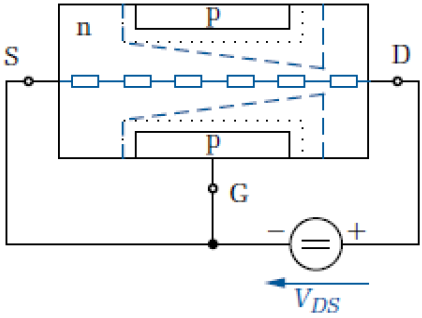
\includegraphics[align=t, width=\columnwidth]{images/fet_aufbau_saettigung.png}
\end{minipage}
\hfill
\begin{minipage}[t]{0.68\columnwidth}
    \begin{itemize}
        \item Für hohes $V_{DS}$ wird leitender Kanal abgeschürt \\
            \textrightarrow\ Strom kann nicht weiter steigen (Stromquelle)
        \item Übergang gest. Widerstand zu Stromquelle @ $V_{DSP}$ \\
        \textrightarrow\ $V_{DSP} = V_{GS} - V_p$ ($V_p =$ Pinch-Off-Spannung)
    \end{itemize}

    $$ I_D = \frac{ I_{DSS}}{V_p^2} \cdot ( V_{GS} - V_p )^2 $$
\end{minipage}

\vspace{0.2cm}
\textbf{Verstärkungsmass Transkonduktanz:}
$$ g_m = \frac{ 2 \cdot I_{DSS}}{V_p^2} \cdot ( V_{GS} - V_p ) = \frac{2}{| V_p |} \cdot \sqrt{I_{DSS} \cdot I_D} \qquad [g_m] = \siemens $$


\subsection{MOS-FETs}

\subsubsection{Aufbau}

\begin{minipage}[t]{0.35\columnwidth}
    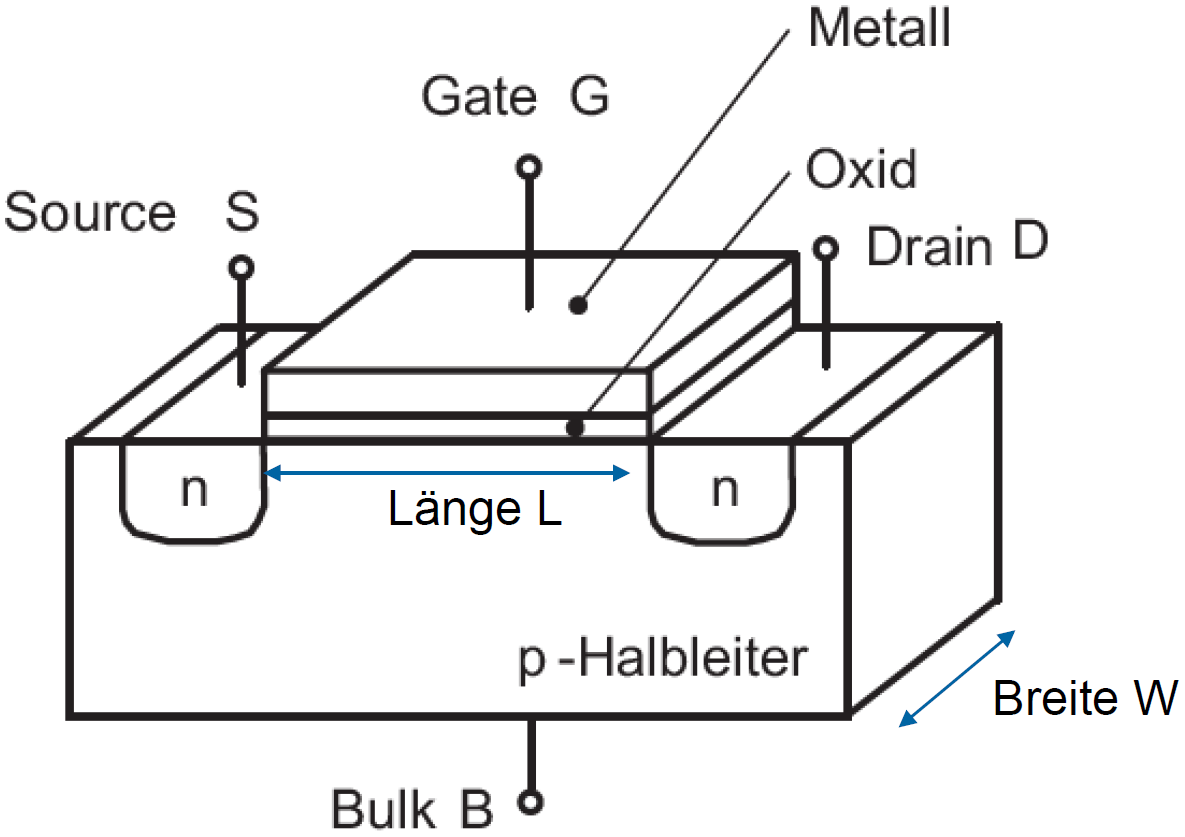
\includegraphics[align=c, width=\columnwidth]{images/mos_fet_aufbau.png}
\end{minipage}
\hfill
\begin{minipage}[c]{0.6\columnwidth}
    \begin{tabular}{l l}
        $L$ & Länge des Transistors  \\
        $W$ & Breite des Transistors \\
        \\
    \end{tabular}

    \begin{itemize}
        \item N-Kanal FET: Drain und Source sind n-dotiert
        \item Kanal ist p-dotiert
    \end{itemize}
\end{minipage}


\subsubsection{Kennlinien}

\begin{minipage}[t]{0.3\columnwidth}
    \textbf{Eingangskennlinie} \\
    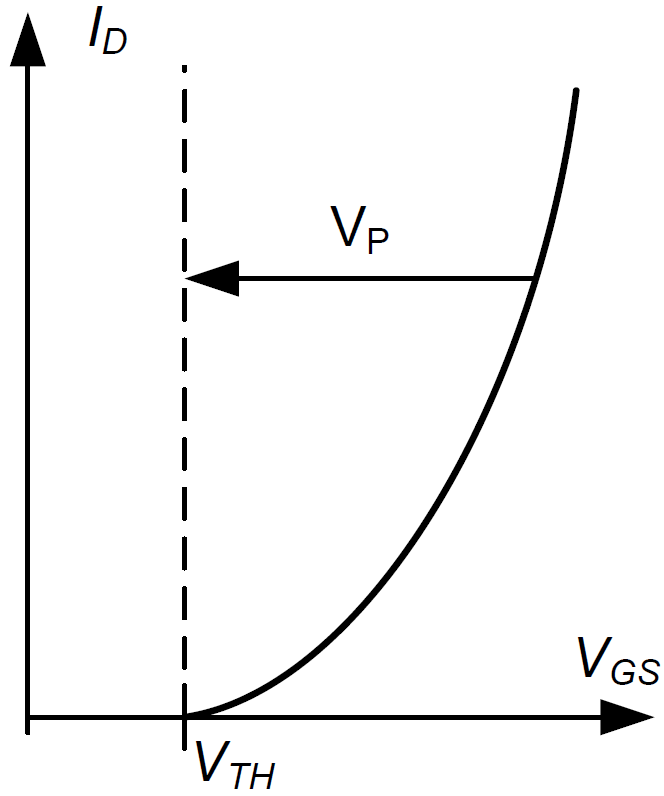
\includegraphics[align=c, width=\columnwidth]{images/mos_fet_eingangskennlinie.png}
\end{minipage}
\hfill
\begin{minipage}[t]{0.6\columnwidth}
    \textbf{Ausgangskennlinien} \\
    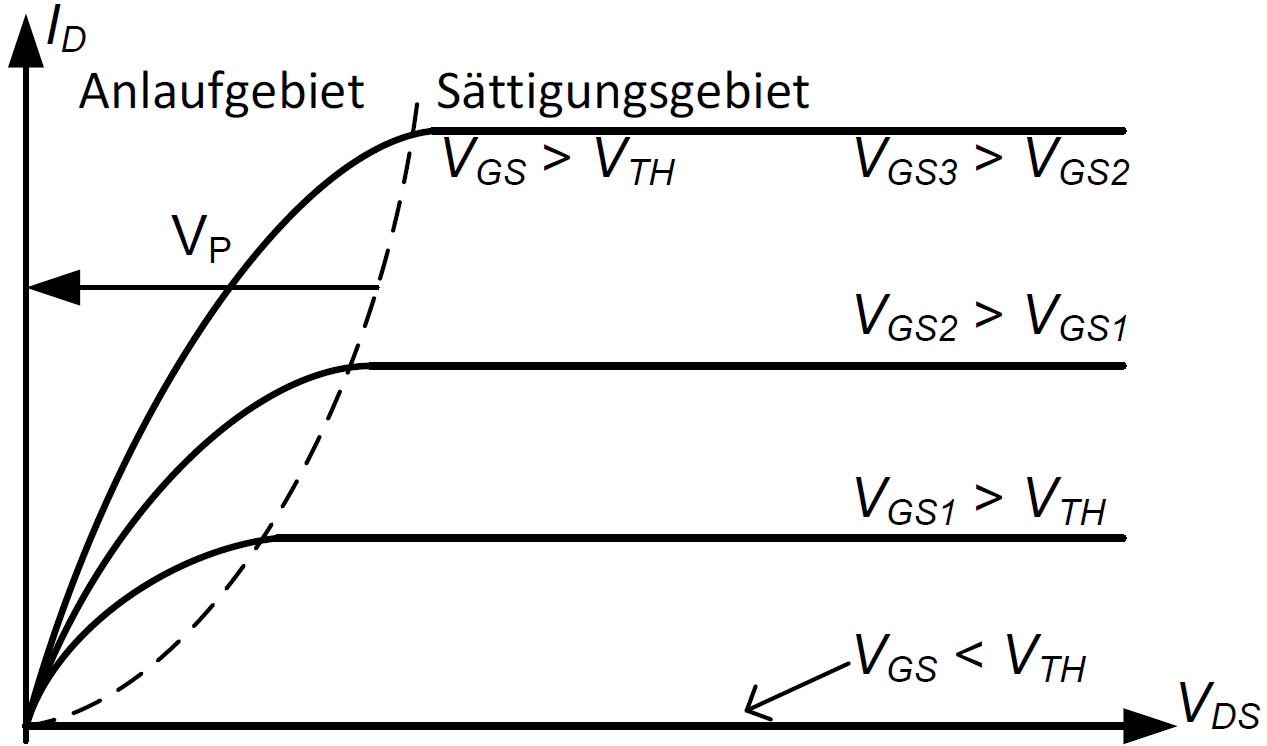
\includegraphics[align=c, width=\columnwidth]{images/mos_fet_ausgangskennlinien.png}
\end{minipage}


\subsubsection{Bereiche}

\begin{itemize}
    \item \textbf{Sperrbereich:} $V_{GS} < V_{TH}$ 
    \item \textbf{Linearer (Widerstands-)Bereich / Anlaufbereich:} $V_{GS} > V_{TH}$
    \item \textbf{Sättigungsbereich (Stromquelle):} $V_{DS} > V_{GS} - V_{TH}$
\end{itemize}

\vspace{0.2cm}

\begin{minipage}[t]{0.48\columnwidth}
    \textbf{Anlaufbereich (Linearer Bereich)}
    $$ I_{D,lin} = \beta \cdot ( V_{GS} - V_{TH} - \frac{V_{DS}}{2} ) \cdot V_{DS} $$
\end{minipage}
\hfill
\begin{minipage}[t]{0.48\columnwidth}
    \textbf{Sättigungsbereich (Stromquelle)}
    $$ I_{D,sat} = \frac{\beta}{2} \cdot ( V_{GS} - V_{TH} )^2 $$
\end{minipage}

% Kanallängenmodulation einfügen?


\subsubsection{Kleinsignal-Ersatzschaltung (MOS-FET)}

\begin{minipage}[t]{0.65\columnwidth}
    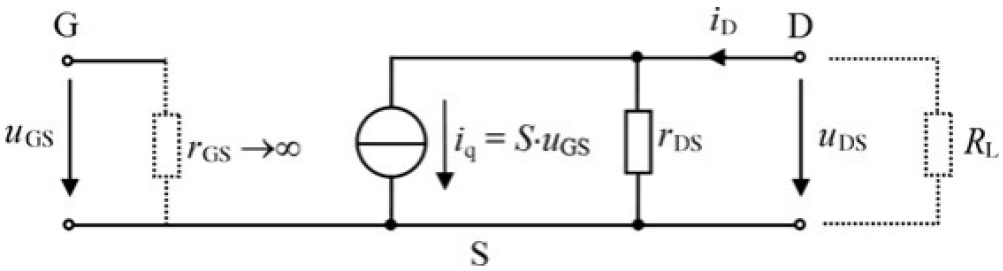
\includegraphics[align=t, width=\columnwidth]{images/mos_fet_kleinsignalersatzschaltung.png}
\end{minipage}
\hfill
\begin{minipage}[t]{0.33\columnwidth}
    $$ \beta = \frac{KP \cdot W}{L} $$
    $$ KP = C_{oc} \cdot \mu_n \approx 100 \frac{\micro \ampere}{\volt^2} $$  % kann man noch verbessern...
\end{minipage}

$$ S = g_m = \beta \cdot (V_{GS} - V_{TH}) = \sqrt{2 \cdot \beta \cdot I_D} = \sqrt{ 2 \cdot \frac{KP \cdot W}{L} \cdot I_D} $$
$$ \frac{1}{r_{DS}} = g_{DS} = \lambda \cdot I_D $$


\subsubsection{Temperaturabhängigkeit der Übrtragungskennlinie}

\begin{minipage}[c]{0.4\columnwidth}
    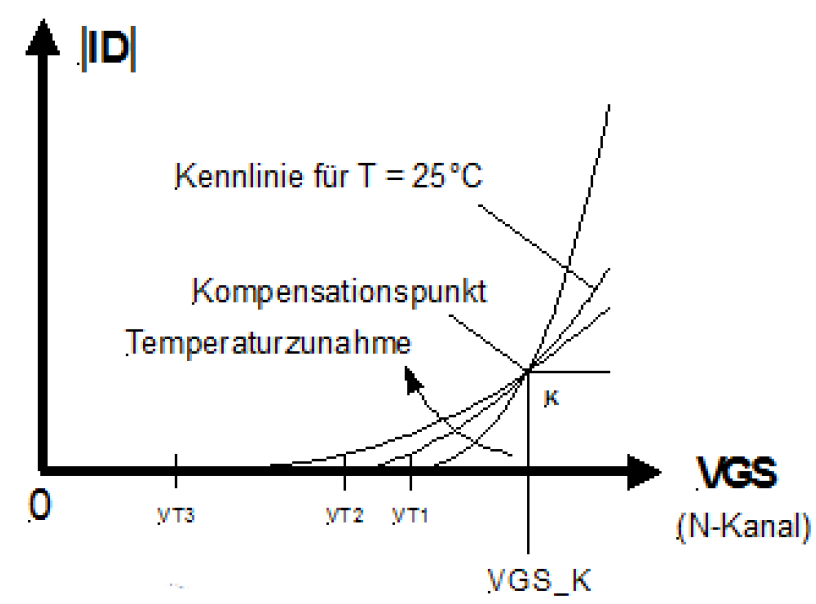
\includegraphics[width= \columnwidth]{images/mos_fet_eingangskennlinie_temperatur.png}
\end{minipage}
\hfill
\begin{minipage}[c]{0.58\columnwidth}
    Für den n-Kanal FET gilt:
    \begin{itemize}
        \item Threshold-Spannung $V_{TH}$ sinkt mit 1-2 $\frac{\micro \volt}{\kelvin}$
        \item $\beta$ sinkt mit steigender Temperatur
        \item Im Kompensationspunkt bleibt $I_D$ für fixes $V_{GS}$ konstant
    \end{itemize}
\end{minipage}

    
\subsection{Verstärkerschaltungen mit FETs}

\subsubsection{Source-Schaltung mit Lastwiderstand}

Um den Arbeitspunkt der Schaltung zu bestimmen, wird die \cbl{Lastgerade von $R_L$} in das
Ausgangskennlinienfeld eingezeichnet

\begin{minipage}[c]{0.4\columnwidth}
    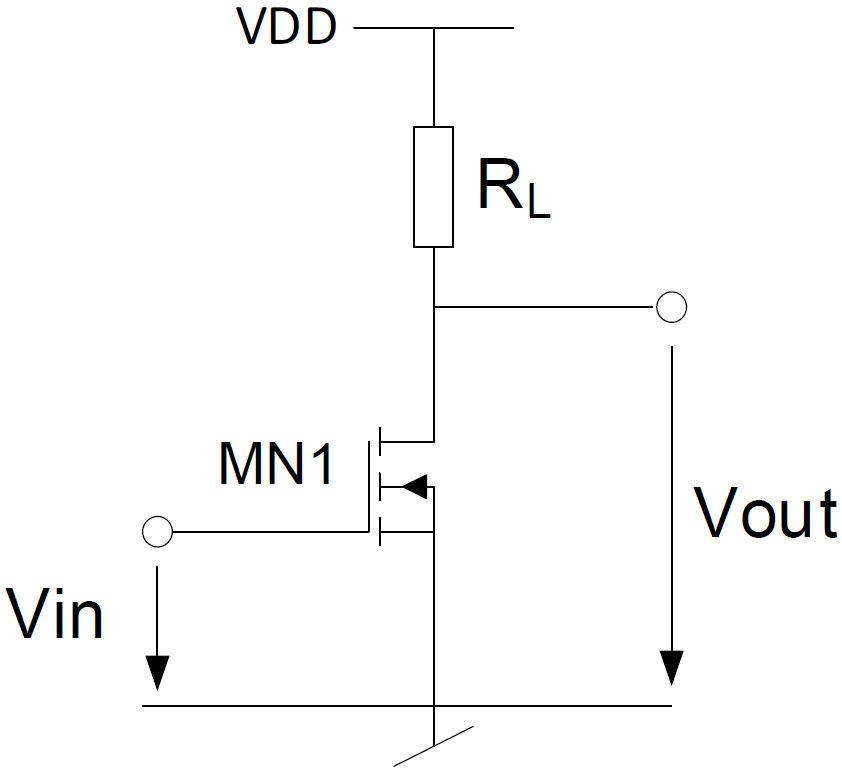
\includegraphics[width=0.9\columnwidth]{images/source_schaltung.png}
\end{minipage}
\hfill
\begin{minipage}[c]{0.5\columnwidth}
    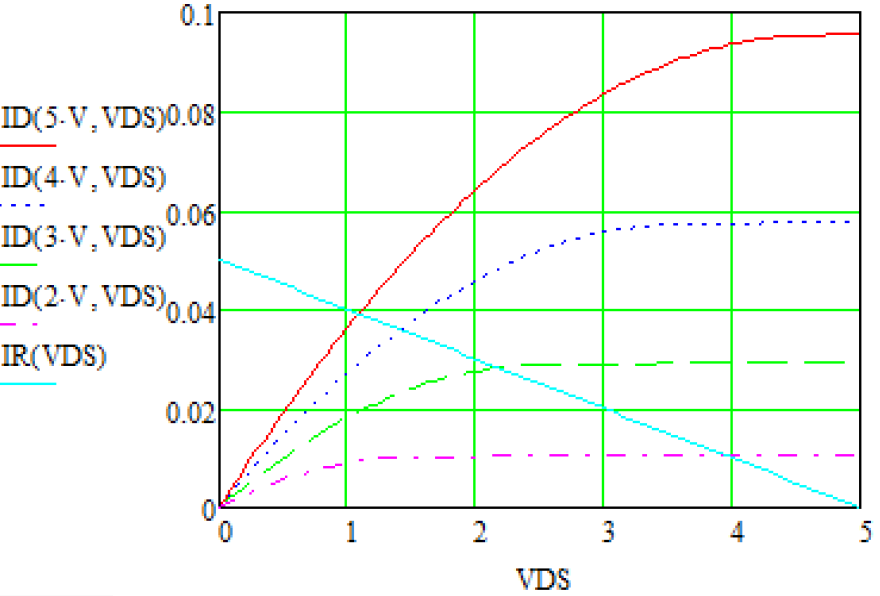
\includegraphics[width=\columnwidth]{images/source_schaltung_lastgerade.png}
\end{minipage}


\subsubsection{Push-Pull / Digitaler Inverter}  % eventuell weglassen

\begin{minipage}[c]{0.35\columnwidth}
    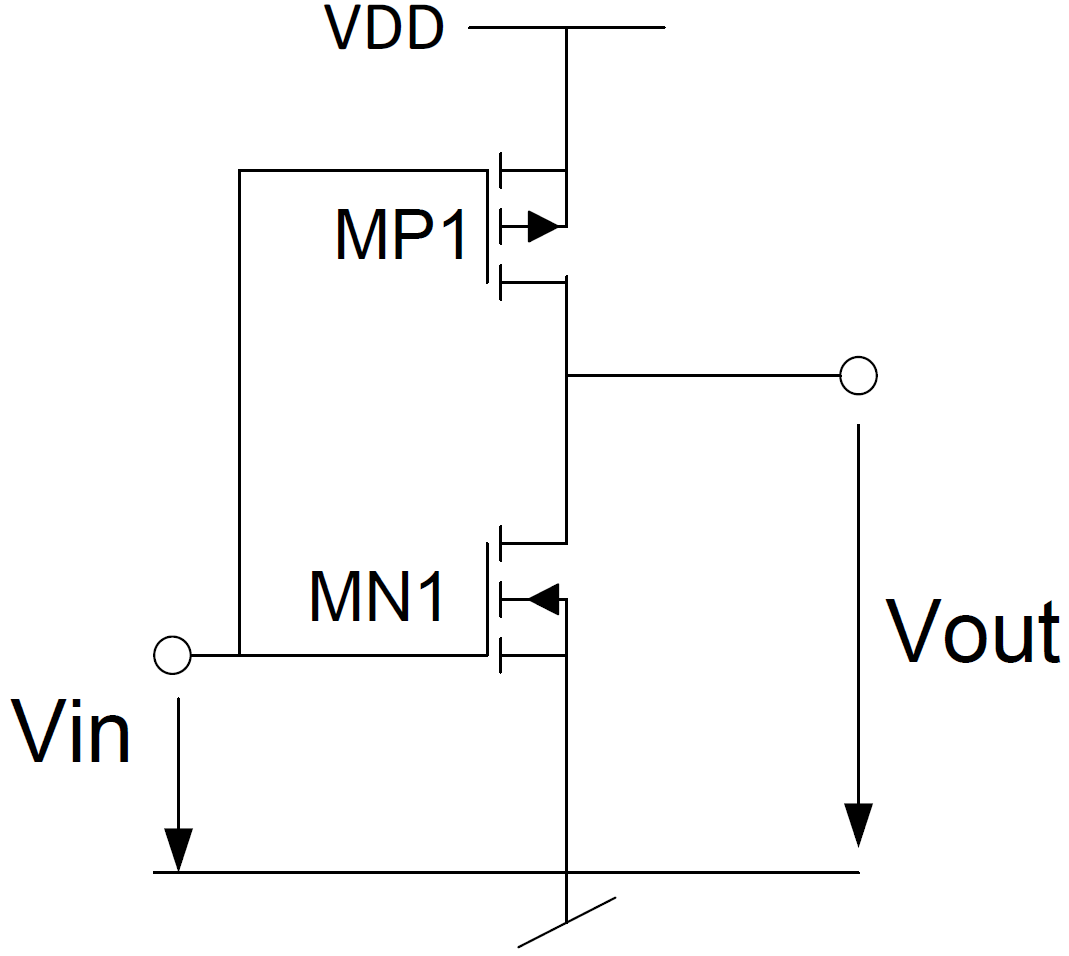
\includegraphics[width=\columnwidth]{images/push_pull_digital_inverter.png}
\end{minipage}
\hfill
\begin{minipage}[c]{0.5\columnwidth}
    \begin{itemize}
        \item $V_{in}$ geht auf NMOS und PMOS
        \item Ermöglicht grössere Verstärkung
    \end{itemize}
        
    \vspace{0.3cm}
    Für $V_{in} \approx \frac{V_{DD}}{2}$ gilt:
    $$ A_{V0} = -(g_{m1} + g_{m2}) \cdot (r_{DS1} || r_{DS2}) $$
\end{minipage}


\subsection{MOS-FET als (Leistungs-)Schalter}
Wenn der FET als Schalter eingesetzt wird, so arbeitet er im \textbf{linearen Bereich} \\
($V_{GS} > V_{TH}$, d.h. $V_{out} < V_{DD} - V_{TH} $)

\begin{minipage}[c]{0.49\columnwidth}
    $$ I_{D,lin} = \beta \cdot ( V_{GS} - V_{TH} - \frac{V_{DS}}{2} ) \cdot V_{DS} $$
    \begin{center}
        
        Schalter geschlossen: $R_{FET} = R_{DS(on)} $
    \end{center}
\end{minipage}
\hfill
\begin{minipage}[c]{0.49\columnwidth}
    $$ r_{DS} = \dfrac{\diff V_{DS}}{\diff I_D} = \frac{1}{\beta \cdot (V_{GS} - V_{TH})}  $$
    \begin{center}
        Schalter offen: $R_{FET} = \infty$ 
    \end{center}
\end{minipage}


\subsubsection{Verlustleistung / Erwärmung}

\begin{minipage}[c]{0.48\columnwidth}
    $$ P_V = R_{DS} * I_{DS}^2 = 0 \, \watt $$
\end{minipage}
\hfill
\begin{minipage}[c]{0.48\columnwidth}
    $$ \Delta T = R_{th} \cdot P_V $$
\end{minipage}


\subsection{Transmission Gate}

\begin{minipage}[c]{0.22\columnwidth}
    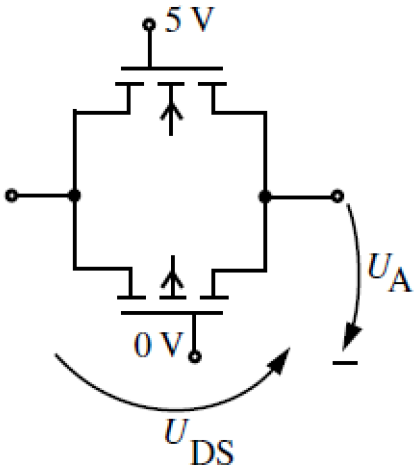
\includegraphics[width=\columnwidth]{images/transmission_gate.png}
\end{minipage}
\hfill
\begin{minipage}[c]{0.68\columnwidth}
    Im Bild links gilt: $V_{DD} = 5 \, \volt$, $V_{SS} = 0 \, \volt$ 

    \begin{itemize}
        \item NMOS (oben) leitet für $V_{in} < V_{DD} - T_{TH,n}$
        \item PMOS (unten) leitet für $V_{in} > V_{SS} - T_{TH,p}$
        \item Source und Drain austauschbar \\
            \textrightarrow\ Strom kann in beide Richtungen fliessen
    \end{itemize}
\end{minipage}